\documentclass[11pt]{article}

\usepackage[margin=1in]{geometry}
\usepackage{graphicx}
\usepackage{booktabs}
\usepackage{hyperref}
\usepackage{amsmath}

\title{Discrete Event Rewards for Training CNN Policies in Learned Visual Worlds}
\author{Anonymous}
\date{}

\begin{document}
\maketitle

\begin{abstract}
Learned visual world models can provide cheap training environments for reinforcement learning, but the reward interface is part of the learned environment.
In earlier Snake pilots, policies optimized continuous learned reward or length predictions and the resulting objectives were hard to interpret.
This paper studies a simpler interface: an action-conditioned world model predicts the next RGB frame plus two discrete events, whether the agent collected the reward item and whether the episode ended in death.
Policies train inside frozen learned worlds using argmax-decoded event rewards, then transfer is measured in the true simulator.
Snake serves as a proof of concept where a single visible frame is nearly Markov and transfer succeeds immediately.
We then extend the same protocol to a more complex Pac-Man-like game with denser visual structure, moving ghosts, randomized connected mazes, and the same discrete event reward.
The central question becomes whether increasing world-model capacity reduces the gap between hallucinated reward and real-simulator reward under a fixed argmax reward interface.
\end{abstract}

\section{Introduction}
Generative interactive environments such as Genie~\cite{bruce2024genie} and real-time game world models such as Matrix-Game 2.0~\cite{he2025matrixgame2} suggest a route to training agents in learned video simulators.
For reinforcement learning, however, the learned simulator is not only a frame predictor.
It also defines rewards, episode endings, and the states that a policy can visit during optimization.
If these interfaces are continuous or poorly matched to the real task, PPO can optimize artifacts that do not exist in the true environment.

We study this issue in small grid games where the true simulator is deterministic and exactly available.
The goal is not to claim that Snake or Pac-Man require world models.
The goal is to build a controlled measurement harness: train a visual world model from simulator data, freeze it, train a CNN policy inside the learned model, and evaluate the same policy in the true simulator.
This directly measures the hallucinated-real transfer gap.

The main design choice is to avoid floating-point learned rewards for control.
The world model predicts event logits.
During policy training, reward is decoded with argmax:
\[
  r_t =
  \begin{cases}
    1 & \text{if the item-collected class wins,}\\
   -1 & \text{if the death class wins,}\\
    0 & \text{otherwise.}
  \end{cases}
\]
This matches the true simulator reward semantics: the agent cannot collect a fractional apple or pellet.

\section{Environments}
\paragraph{Snake.}
Snake is rendered as a $128 \times 128$ RGB board with no HUD, score text, or visual episode-status overlay.
The image contains the board, rocks, apples, and snake.
A single frame exposes the snake body, apples, rocks, and head orientation, so context length one is close to Markov.
The only small ambiguity is that ignored reverse actions depend on current direction, which is visually encoded by the head/body arrangement in almost all states.

\begin{figure}[t]
  \centering
  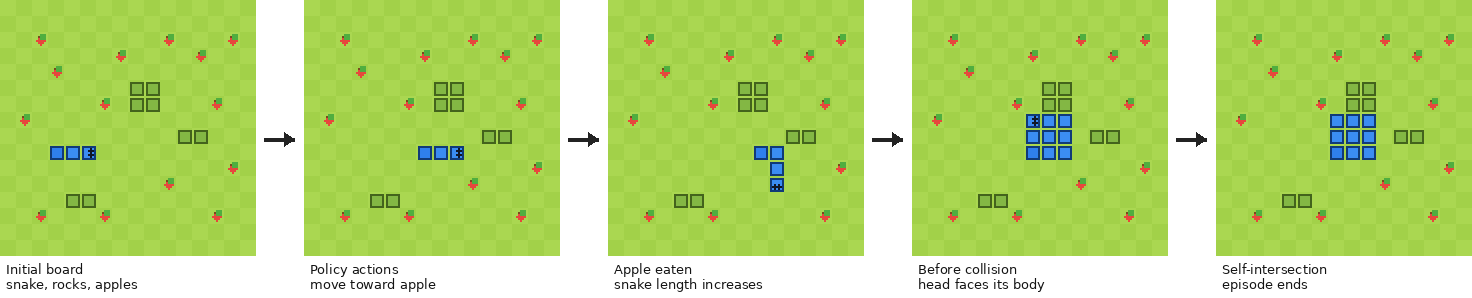
\includegraphics[width=\linewidth]{figures/snake_environment_sequence.png}
  \caption{Snake simulator sequence used as the proof-of-concept environment. Frames show the initial state, movement, apple collection, and death by self-intersection.}
  \label{fig:snake-env}
\end{figure}

\paragraph{Pac-Man.}
Pac-Man is a harder extension rendered as a $256 \times 256$ RGB board.
The map contains blue maze walls, pellets, Pac-Man, and four colored ghosts.
Maps can be randomized, but pellets are placed only on cells reachable from the player start by flood fill.
This prevents invalid maps where isolated pellets make success impossible.
Unlike Snake, one frame may not fully specify ghost motion history or recent action effects, so Pac-Man is a stronger test of whether a context-one world model can support policy training.

\begin{figure}[t]
  \centering
  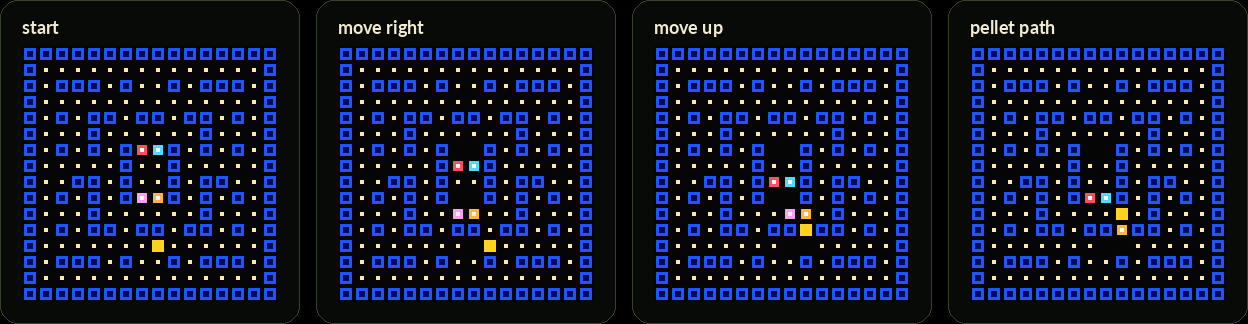
\includegraphics[width=\linewidth]{figures/pacman_environment_sequence.png}
  \caption{Pac-Man-like simulator frames. The same discrete event interface is used: pellet collected, death, and next RGB frame.}
  \label{fig:pacman-env}
\end{figure}

\begin{figure}[t]
  \centering
  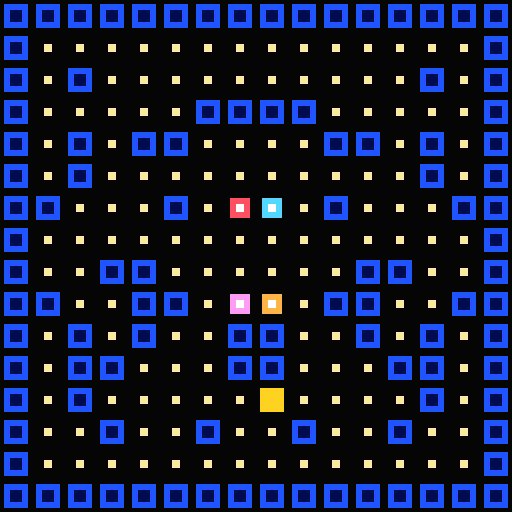
\includegraphics[width=0.55\linewidth]{figures/pacman_random_map.png}
  \caption{Example randomized Pac-Man map. The generator accepts only connected maps with a large reachable pellet region.}
  \label{fig:pacman-random}
\end{figure}

\section{World model and policy training}
The event world model is action-conditioned and autoregressive.
Given the previous RGB frame $x_t$ and action $a_t$, it predicts
\[
  \hat{x}_{t+1},\quad \hat{e}_{t+1},\quad \hat{d}_{t+1},
\]
where $\hat{x}_{t+1}$ is the next frame, $\hat{e}_{t+1}$ are item-collected logits, and $\hat{d}_{t+1}$ are death logits.
We train models at several capacities: a tiny model, a roughly one-million-parameter model, a roughly two-million-parameter model, and for Snake a larger five-million-parameter model used for the final visualization.
All policy experiments in this paper use the hard argmax event decoder.

CNN policies are trained with PPO inside the frozen learned world.
At each imagined step, the policy observes the current predicted RGB frame, samples an action, and the world model predicts the next frame and event logits.
The PPO reward is the hard event reward above.
Episodes terminate when the argmax death class fires or when a maximum rollout length is reached.
After training, the same CNN policy is evaluated in the true simulator without modification.

\section{Snake proof of concept}
Snake provides the basic sanity check: can a CNN trained only in a learned visual world transfer when the reward interface is discrete and faithful to the real simulator?
Table~\ref{tab:snake-random} summarizes the main argmax-event result on fixed and randomized layouts.
The key observation is that frozen learned-world training transfers immediately under the hard event interface.
No additional real-rollout fine-tuning is needed for this setting.

\begin{table}[t]
  \centering
  \begin{tabular}{llrrrrr}
\toprule
Decoder & Layout & Hall. return & Real return & Real apples & Death & Win \\
\midrule
hard & fixed & 9.04 & 13.00 & 13.00 & 0.00 & 1.00 \\
hard & random apples & 9.04 & 11.02 & 11.16 & 0.14 & 0.42 \\
hard & random start apples & 9.04 & 11.55 & 11.62 & 0.07 & 0.45 \\
prob & fixed & 9.07 & 13.00 & 13.00 & 0.00 & 1.00 \\
prob & random apples & 9.07 & 12.04 & 12.10 & 0.06 & 0.57 \\
prob & random start apples & 9.07 & 11.62 & 11.69 & 0.07 & 0.54 \\
\bottomrule
\end{tabular}

  \caption{Snake policy transfer with hard argmax event rewards. The ``prob'' rows are retained as an ablation of reward decoding, while all final-policy claims use hard argmax rewards.}
  \label{tab:snake-random}
\end{table}

\begin{table}[t]
  \centering
  \begin{tabular}{lrrrr}
\toprule
Policy & Hard real apples & Prob. real apples & Hard gap & Prob. gap \\
\midrule
small & 13.00 & 13.00 & -6.69 & -4.79 \\
medium & 12.00 & 13.00 & -3.29 & -5.87 \\
large & 13.00 & 13.00 & -5.11 & -4.63 \\
\bottomrule
\end{tabular}

  \caption{Snake hard-event versus probability-decoded event rewards across policy sizes. The hard setting is the paper's intended interface; probability decoding is included to show why reward decoding is part of the environment.}
  \label{tab:snake-hard-prob}
\end{table}

\begin{figure}[t]
  \centering
  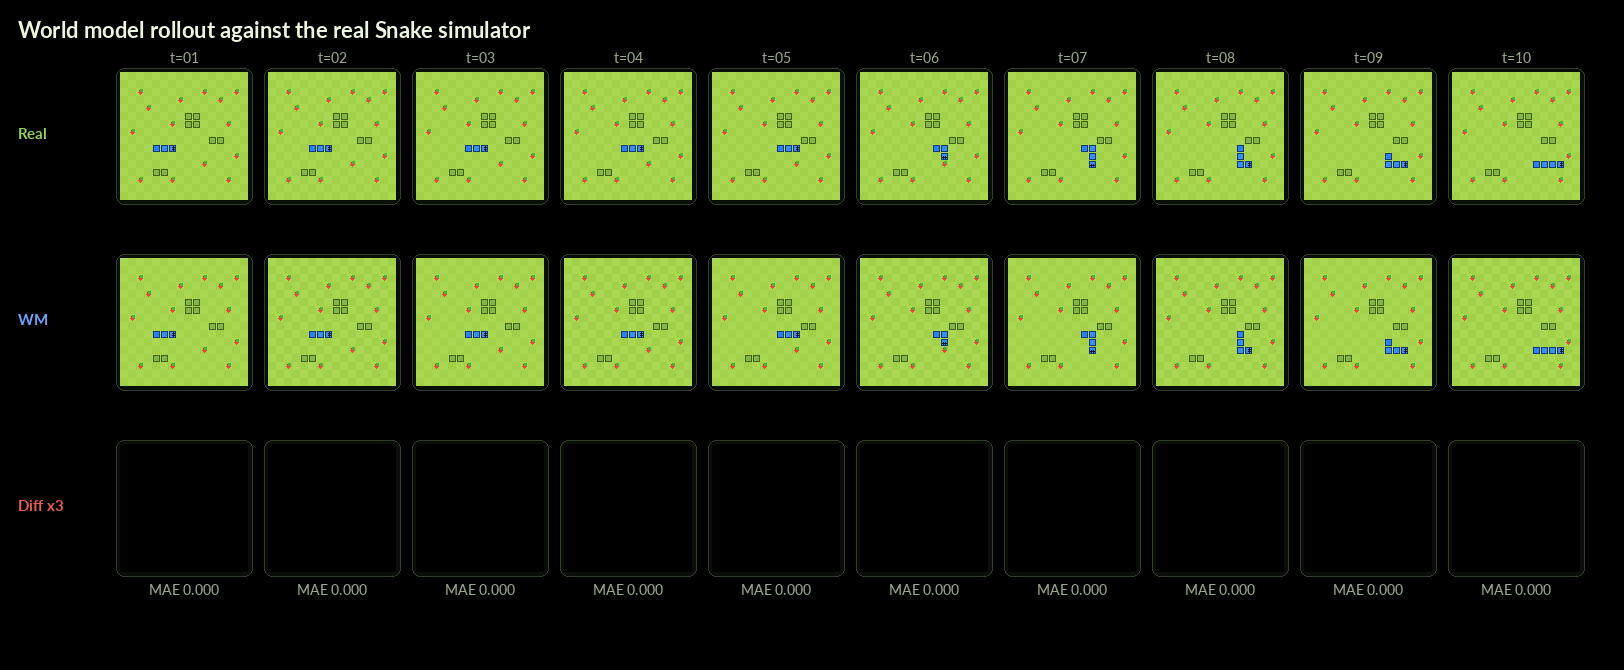
\includegraphics[width=\linewidth]{figures/wm_vs_sim_rollout.png}
  \caption{Snake real simulator versus autoregressive world-model rollout. The learned model is accurate enough over short horizons for policy optimization under hard event rewards.}
  \label{fig:snake-rollout}
\end{figure}

\begin{figure}[t]
  \centering
  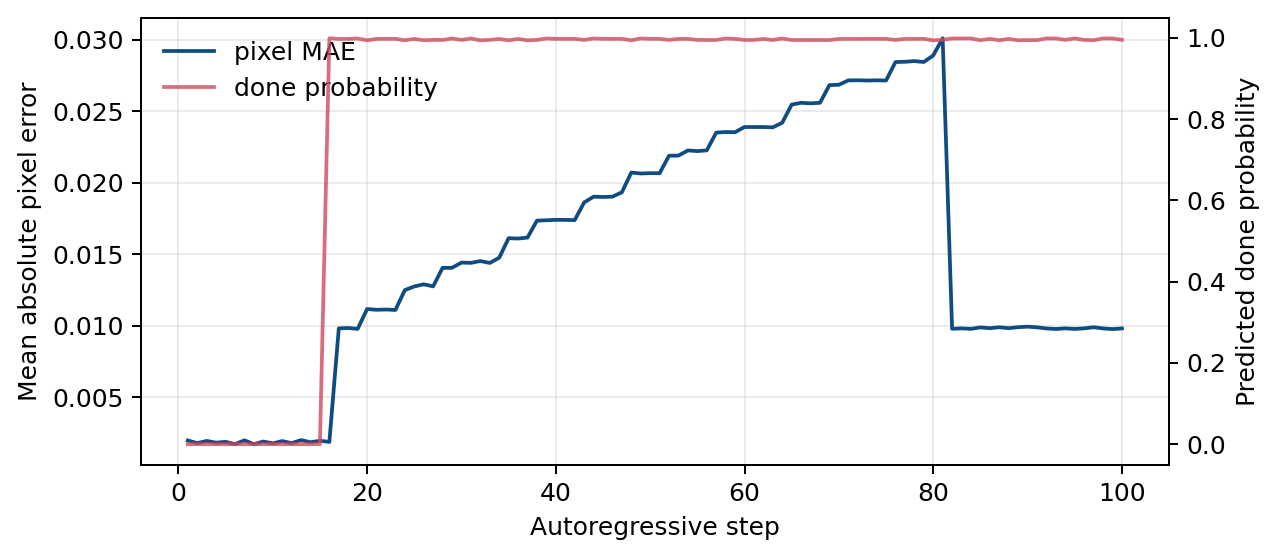
\includegraphics[width=0.82\linewidth]{figures/wm_drift_curve.png}
  \caption{Snake world-model drift during an autoregressive rollout. Frame error remains low over the first steps used in the visualization.}
  \label{fig:snake-drift}
\end{figure}

\section{Pac-Man extension}
Pac-Man tests the same interface in a game with denser images, more objects, and moving adversaries.
The experiment matrix trains a random-map Pac-Man dataset, event world models of different sizes, and small CNN policies inside each frozen world model.
All Pac-Man policy training uses hard argmax pellet rewards and hard argmax death termination.
No floating-point reward head or length head is used for control.

\begin{table}[t]
  \centering
  \begin{tabular}{llrrrr}
\toprule
World model & Eval & Return & Pellets & Steps & Death \\
\midrule
tiny & hallucinated & 244.07 & 244.15 & 245.9 & 0.04 \\
tiny & real & 0.96 & 1.60 & 187.3 & 0.64 \\
wm\_1m & hallucinated & 1.62 & 1.75 & 223.4 & 0.13 \\
wm\_1m & real & 1.00 & 1.70 & 155.8 & 0.70 \\
wm\_2m & hallucinated & 1.04 & 1.19 & 217.8 & 0.15 \\
wm\_2m & real & 0.14 & 0.78 & 185.6 & 0.64 \\
\bottomrule
\end{tabular}

  \caption{Pac-Man hallucinated and real-simulator evaluation by world-model size. This table is generated from the matrix runner after each world-model/policy cell completes.}
  \label{tab:pacman}
\end{table}

\begin{figure}[t]
  \centering
  
\includegraphics[width=0.78\linewidth]{figures/pacman_argmax_transfer.png}
  \caption{Pac-Man real-simulator transfer after training the CNN inside each frozen argmax-event world model. The red markers show death rate.}
  \label{fig:pacman-transfer}
\end{figure}

\begin{figure}[t]
  \centering
  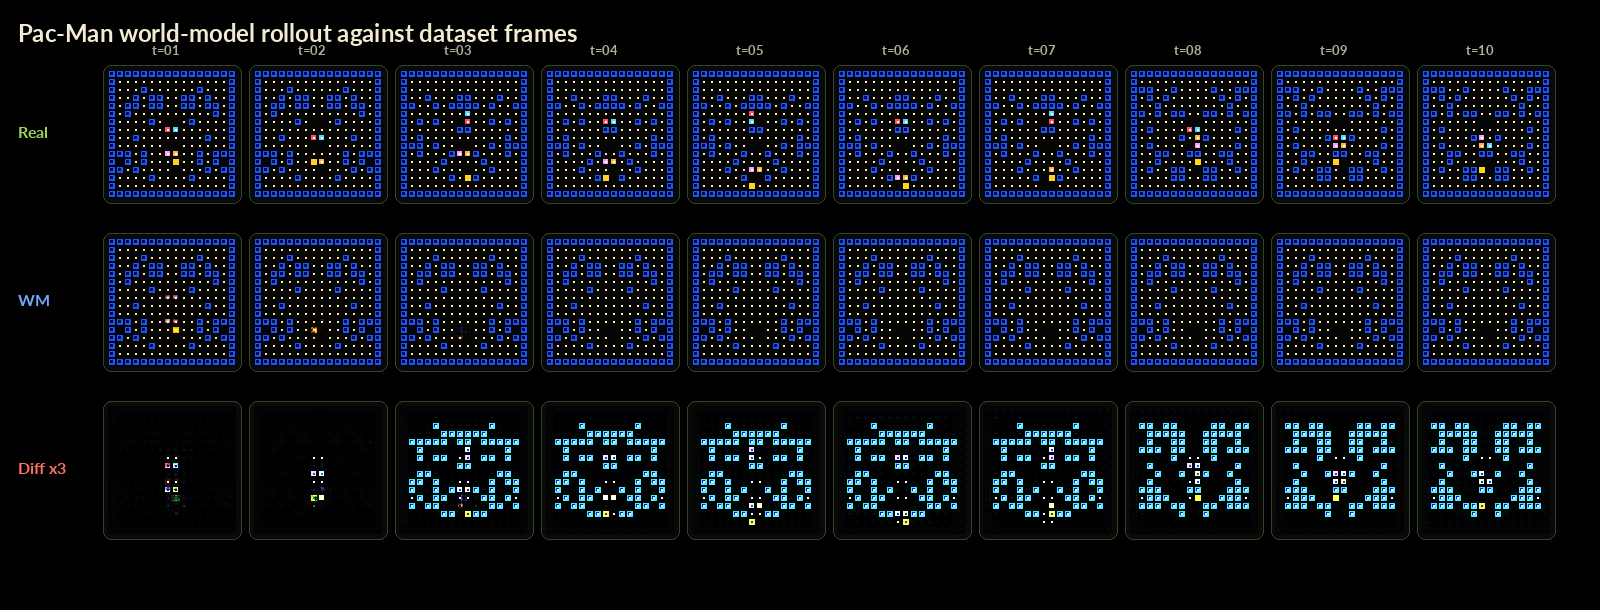
\includegraphics[width=\linewidth]{figures/pacman_wm_vs_sim_rollout.png}
  \caption{Pac-Man dataset frames compared with an autoregressive tiny-world-model rollout under the same action sequence. The tiny model reconstructs local visual structure but drifts over several steps.}
  \label{fig:pacman-rollout}
\end{figure}

\begin{figure}[t]
  \centering
  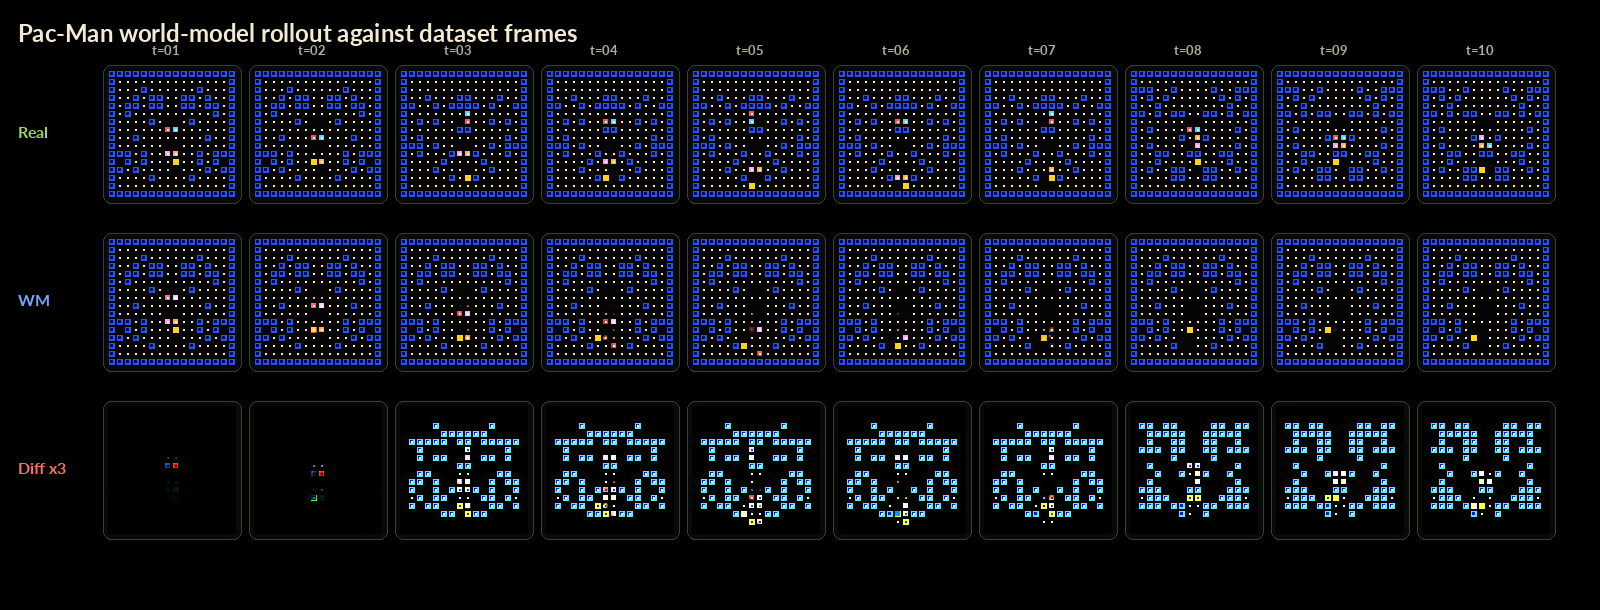
\includegraphics[width=\linewidth]{figures/pacman_wm2_vs_sim_rollout.png}
  \caption{Pac-Man dataset frames compared with an autoregressive two-million-parameter world-model rollout under the same action sequence. The larger model improves short-horizon visual consistency, but policy transfer remains weak.}
  \label{fig:pacman-rollout-wm2}
\end{figure}

The result is capacity-based but not solved.
With the tiny Pac-Man world model, PPO discovers a strongly model-specific strategy: hallucinated evaluation reports about 244 predicted pellets per episode, while real random-map evaluation collects about 1.6 pellets and dies in 64\% of episodes.
This is model exploitation despite hard argmax rewards.
Increasing capacity to the one-million- and two-million-parameter models removes most of the hallucinated reward explosion, but it does not produce a strong transferred Pac-Man policy.
The one-million-parameter policy collects about 1.7 pellets in the real simulator, and the two-million-parameter policy collects about 0.8 pellets.
Thus the larger models are less obviously exploitable, but the learned worlds still are not good enough training environments for Pac-Man.

\section{Discussion}
The Snake result changes the original framing.
The clearest lesson is not that CNN policies inevitably exploit learned Snake worlds.
Rather, the reward interface strongly determines what environment PPO is optimizing.
When the policy receives continuous learned rewards or length predictions, the objective can encode values that never occur in the real simulator.
When the policy receives argmax-decoded item and death events, the learned environment is much closer to the real task.

This does not remove model exploitation as a concern.
It moves the question to world-model capacity and domain complexity.
Snake is almost fully observable from one frame, and the learned model transfers well.
Pac-Man introduces moving ghosts, randomized mazes, and more complex visual dynamics.
The relevant failure mode is therefore no longer fractional reward hacking, but policy optimization against an underpowered learned transition model.
The tiny Pac-Man model shows the old failure mode in a cleaner form: even after removing fractional rewards, PPO can still exploit incorrect learned dynamics.
The larger Pac-Man models show a different outcome: lower hallucinated reward, lower transfer gap, and still poor real performance.
For this paper, that negative result is important because it separates ``the reward interface is wrong'' from ``the learned simulator is not yet accurate enough for control.''

\section{Limitations}
Both games are small deterministic simulators.
Argmax event rewards are natural here because item collection and death are discrete and easy to label.
Richer domains may have ambiguous rewards or partial observability that require memory, recurrent policies, or multi-frame context.
For Pac-Man especially, context one may be insufficient if ghost direction or timing cannot be inferred from a single image.
The paper should therefore be read as a controlled case study of reward-interface design and model capacity, not as a general claim that frozen visual world models solve model-based RL.

\section{Reproducibility}
The repository contains dataset generation, world-model training, PPO policy training, real-simulator evaluation, visual export scripts, and W\&B logging.
Snake and Pac-Man use the same indexed transition format and the same event-world-model training code.
The Pac-Man matrix runner is \texttt{scripts/run\_pacman\_argmax\_matrix.sh}.
All logged runs use hard argmax event rewards for the final policy-training protocol.

\bibliographystyle{plain}
\bibliography{references}
\end{document}
